\documentclass[10pt,a4paper]{article}
\usepackage[T1]{fontenc}
\usepackage[brazil]{babel}
\usepackage[utf8]{inputenc}

\newcommand{\red}[1]{\textcolor{red}{#1}}

\usepackage{ae,aecompl}
\usepackage{pslatex}
\usepackage{epsfig}
\usepackage{geometry}
\usepackage{url}
\usepackage{textcomp}
\usepackage{ae}
\usepackage{subfig}
\usepackage{indentfirst}
\usepackage{textcomp}
\usepackage{color}
\usepackage{setspace}
\usepackage{verbatim}
\usepackage{multicol}

\usepackage{listings}
\lstset{language=C}
\usepackage{listings}
\lstset{
  basicstyle=\footnotesize\ttfamily, % Standardschrift
  numbers=left,               % Ort der Zeilennummern
  numberstyle=\tiny,          % Stil der Zeilennummern
  % stepnumber=2,               % Abstand zwischen den Zeilennummern
  numbersep=5pt,              % Abstand der Nummern zum Text
  tabsize=2,                  % Groesse von Tabs
  extendedchars=true,         %
  breaklines=true,            % Zeilen werden Umgebrochen
  classoffset=0,
  keywordstyle=\color{blue},
  classoffset=1,
  morekeywords={factor},keywordstyle=\color{red},
  classoffset=0,
  % frame=b,         
  % keywordstyle=[1]\textbf,    % Stil der Keywords
  % keywordstyle=[2]\textbf,    %
  % keywordstyle=[3]\textbf,    %
  % keywordstyle=[4]\textbf,   \sqrt{\sqrt{}} %
  stringstyle=\color{green}\ttfamily, % Farbe der String
  showspaces=false,           % Leerzeichen anzeigen ?
  showtabs=false,             % Tabs anzeigen ?
  xleftmargin=17pt,
  framexleftmargin=17pt,
  framexrightmargin=5pt,
  framexbottommargin=4pt,
  % backgroundcolor=\color{lightgray},
  showstringspaces=false      % Leerzeichen in Strings anzeigen ?        
}
\lstloadlanguages{Java}



% Definindo o espaçamento entre linhas para 1.5
% Relatório parcial deve ter espaçamento simples
\linespread{1.5}

\geometry{ 
  a4paper,	% Formato do papel
  tmargin=30mm,	% Margem superior
  bmargin=30mm,	% Margem inferior
  lmargin=20mm,	% Margem esquerda
  rmargin=20mm,	% Margem direita
  footskip=20mm	% Espaço entre o rodapé e o fim do texto
}
%  ABACO -- Conjunto de macros para desenhar o 'abaco

%  Desenho original de Hans Liesenberg

%  Macros de Tomasz Kowaltowski

%  DCC -- IMECC -- UNICAMP

%  Mar,co de 1988  --  Vers~ao 1.0

% Ajustado para LaTeX da SUN -- Mar,co de 1991

% ---------------------------------------------------------

%  Chamada:   \ABACO{d1}{d2}{d3}{d4}{esc}
%             com:  di's -- os quatro d'igitos;
%	           esc  -- fator de escala

% ---------------------------------------------------------

%  DEFINI,C~OES AUXILIARES

% ---------------------------------------------------------


%  Forma o d'igito pequeno (0 ou 1)

\newcommand{\ABACODP}[1]{%
%
\thicklines
%    
\begin{picture}(8,0)
    \ifcase#1{   %  caso 0
       \put(0,0)    {\line(1,0){4}}
       \multiput(5,0)(2,0){2}{\oval(2,4)}}
    \or{         %  caso 1
       \put(2,0)    {\line(1,0){4}}
       \multiput(1,0)(6,0){2}{\oval(2,4)}}
    \fi
\end{picture}
    } % \ABACODP

% Forma o d'igito grande (0 a 4)

\newcommand{\ABACODG}[1]{%
%
\thicklines
%    
\begin{picture}(14,0)
    \ifcase#1{   % caso 0
       \multiput(1,0)(2,0){5}{\oval(2,4)}}
       \put(10,0)   {\line(1,0){4}}
    \or{         % caso 1
       \multiput(1,0)(2,0){4}{\oval(2,4)}}
       \put(8,0)   {\line(1,0){4}}
       \put(13,0)   {\oval(2,4)}
    \or{         % caso 2
       \multiput(1,0)(2,0){3}{\oval(2,4)}
       \put(6,0)   {\line(1,0){4}}
       \multiput(11,0)(2,0){2}{\oval(2,4)}}
    \or{         % caso 3
       \multiput(1,0)(2,0){2}{\oval(2,4)}
       \put(4,0)   {\line(1,0){4}}
       \multiput(9,0)(2,0){3}{\oval(2,4)}}
    \or{         % caso 4
       \put(1,0)  {\oval(2,4)}}
       \put(2,0)   {\line(1,0){4}}
       \multiput(7,0)(2,0){4}{\oval(2,4)}
    \fi
\end{picture}
    } % \ABACODG
       
% Forma um d'igito (0 a 9)

\newcommand{\ABACOD}[1]{%
%
    \ifnum#1>9
       \errmessage{#1: Argumento invalido para ABACO}
    \fi
    \ifnum#1<0
       \errmessage{#1: Argumento invalido para ABACO}
    \fi
%
\begin{picture}(24,0)
%    
    \ifnum#1<5
       \put(16,0) {\ABACODP{0}}
    \else   
       \put(16,0) {\ABACODP{1}}
    \fi
%    
    \ifnum#1<5
       \put(0,0)  {\ABACODG{#1}}
    \else
       \ifcase#1\or \or \or \or
          \or  \put(0,0)  {\ABACODG{0}}
          \or  \put(0,0)  {\ABACODG{1}}
          \or  \put(0,0)  {\ABACODG{2}}
          \or  \put(0,0)  {\ABACODG{3}}
          \or  \put(0,0)  {\ABACODG{4}}
       \fi
    \fi   
\end{picture}
    } % \ABACOD
    
% -------------------------------------------------

%  DEFINI,C~AO PRINCIPAL
    
\newcommand{\ABACO}[5]{%
    \setlength{\unitlength}{#5mm}
%
    \thinlines
%   
\begin{picture}(28,25)
%   
% moldura
%
% externa
%
        \put(0,0)            {\line(0,1){25}}
        \put(0,0)            {\line(1,0){28}}
        \put(28,0)           {\line(0,1){25}}
        \put(0,25)           {\line(1,0){28}}
% interna
        \put(2,2)            {\line(0,1){21}}
	\put(26,2)           {\line(0,1){21}}
	\put(16,2)           {\line(0,1){21}}
	\put(18,2)           {\line(0,1){21}}
	\put(2,2)            {\line(1,0){14}}
	\put(16,2)           {\line(1,-1){1}}
	\put(17,1)           {\line(1,1){1}}
	\put(18,2)           {\line(1,0){8}}
	\put(2,23)           {\line(1,0){14}}
	\put(16,23)          {\line(1,1){1}}
	\put(17,24)          {\line(1,-1){1}}
	\put(18,23)          {\line(1,0){8}}
	\put(0,0)            {\line(1,1){2}}
	\put(0,25)           {\line(1,-1){2}}
	\put(28,0)           {\line(-1,1){2}}
	\put(28,25)          {\line(-1,-1){2}}
%
%   
% d'igitos
%
%   
       \put(2,20)  {\ABACOD{#1}}
       \put(2,15)  {\ABACOD{#2}}
       \put(2,10)  {\ABACOD{#3}}
       \put(2,5)   {\ABACOD{#4}}
%      
\end{picture}
    } % \ABACO
    
 
\renewcommand{\thetable}{\Roman{table}}
\newcommand{\x} {$\bullet$}


\begin{document}

% CAPA
\begin{titlepage}
  \thispagestyle{empty}
  \begin{center} {\large \textbf{UNIVERSIDADE~ESTADUAL~DE~CAMPINAS}} \end{center}
  \begin{center} {\large INSTITUTO~DE~COMPUTAÇÃO}                    \end{center}
  \vspace{0.1cm}
  \begin{center}
    \begin{minipage}[tl]{31mm}
      \ABACO{1}{9}{6}{9}{1}
    \end{minipage}
  \end{center}
  \vspace{0.3cm}
  \begin{center} 
    {\large \textsc{Servidor de Agenda baseado em socket UDP
      }} 
    \\\vspace{0.5cm}
    {\textsl{Relatório do segundo laboratório de MC823}}
    \\\vspace{1cm}
    \begin{tabular}{ll}
      \textbf{Aluno}:        Marcelo~Keith~Matsumoto   &  \textbf{RA}:       085937 \\
      \textbf{Aluno}:        Tiago~Chedraoui~Silva    &   \textbf{RA}:       082941 \\
      
    \end{tabular}
  \end{center}
  \vspace{0.5cm}

  \begin{abstract}

    The Java Remote Method Invocation (RMI) system allows an object running in one Java virtual machine to invoke methods on an object running in another Java virtual machine. RMI provides for remote communication between programs written in the Java programming language.

  \end{abstract}

\end{titlepage} 
% Sumário
\tableofcontents

\newpage


% -----------------------------------------------------------------------------%
\section{Objetivo}
% -----------------------------------------------------------------------------%
O objetivoterceiro projeto de laboratório de teleprocessamento e redes é
comparar duas implementações distintas do modelo cliente-servidor: Java
RMI (Remote Method Invocation) e socket TCP. 
É de suma importância que utilizando a tecnologia Java RMI, cria-se
uma agenda, para possibilitar uma comparação
com a mesma agenda em socket TCP, criada anteriormente no projeto 1.

\subsection{Teoria}
Java RMI é uma das abordagens da tecnologia Java, construída para prover as
funcionalidade de uma plataforma de objetos distribuídos e com sua API (Application
Programming Interface) especificada pelo pacote java.rmi e seus subpacotes. A
arquitetura RMI viabiliza a interação de um objeto ativo em uma máquina virtual Java com
objetos de outras máquinas virtuais Java.

Aplicações que utilizam objetos distribuídos precisam das realizar as seguintes ações:
\begin{description}
\item[Localização de objetos remotos] aplicações podem usar vários
  métodos para obter referências a objetos remotos. Ex: utilizar  RMI registry
\item [Comunicação com objetos remotos] Detalhes da comunicação entre
  objeto remotos são gerenciados pelo RMI, ou seja para o programador
  chamadas remotas são similares a chamadas de métodos.
\item [Carregamento de definições de classes para objetos móveis]
  RMI prove mecanismos para carregar a definição de classes para um
  objeto assim como para transmitir seus dados
\end{description}

Para o desenvolvimento de uma aplicação cliente-servidor em Java RMI, são
necessários um cliente e um para o servidor e a
execução do serviço de registro de RMI (RMI registry)(Ver figura
figura \ref{f1}). Um servidor, em geral, instancia
objetos remotos, referencia estes objetos e liga-os em uma determinada porta através de
um bind, aguardando nesta porta os clientes invocarem os métodos destes objetos. Um
cliente, em geral, referência remotamente um ou mais objetos remotos de um servidor, e
invoca os métodos destes objetos. Os mecanismos pelos quais o cliente e o servidor se
comunicam e trocam dados são fornecidos pelo Java RMI. O serviço de registro de RMI é
uma implementação de um serviço de nomes para RMI, no qual cada serviço
disponibilizado na plataforma é registrado através de um nome de serviço, ou seja, uma
string única para cada objeto o qual implementa serviços em RMI.

\begin{figure}[h!]
  \begin{center}
    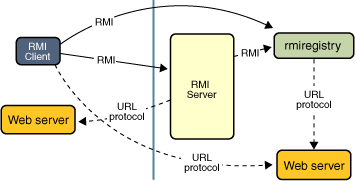
\includegraphics[scale=0.7]{rmi-img.png}
    \caption{Aplicação distribuida RMI que usa o RMI registry para obter a
      referência para um objeto remoto.}
    \label{f1}
  \end{center}
\end{figure}


% -----------------------------------------------------------------------------%
\section{Servidor de agenda}
% -----------------------------------------------------------------------------%
Para criar uma aplicação distribuída usando a tecnologia RMI deve-se
projetar e implementar as componentes da aplicação.
Primeiro define as interfaces,depois, baseado nas interfaces,
implementa-se os objetos e posteriormente o cliente.

O sistema implementado, uma agenda distribuída, se baseia numa comunicação
cliente-servidor. Nele o servidor possui todas as informações da
agenda que estão armazenadas em um banco de dados,
assim como as opções de interações com os dados que são apresentadas
aos clientes em formas de um menu.
O cliente só escolhe alguma opção de interação com os dados de
acordo com menu.


\subsection{Menu inicial}
No menu inicial pode-se:

\begin{itemize}
\item Logar
\item Criar novo usuário
\item Sair
\end{itemize}

\subsubsection{Login}
O servidor pede ao usuário o nome de usuário, caso o nome estiver no
banco de dados ele pede uma senha que é comparada ao valor do banco de
dados, se o usuário não existir é avisado sobre a inexistência, se a
senha não conferir é avisado que a senha não confere, caso contrário o
usuário consegue logar no sistema, e o servidor recupera sua agenda (cada
usuário possui sua agenda).


\subsubsection{Novo usuário}
O servidor pede um nome de usuário, o servidor verifica se o nome já
não existe, se não existir pede a senha e armazena o usuário no
sistema, assim como cria uma agenda vazia para o mesmo.

\subsection{Menu usuário}
Dentre as possibilidades de interações para um usuário logado tem-se:

\begin{itemize}
\item Inserção de um compromisso que possui um nome, dia, hora, e minuto. 
\item Remoção de um compromisso através de seu nome
\item Pesquisa de compromisso por dia
\item Pesquisa de compromisso por dia e hora
\item Ver todos os compromisso de mês de abril
\end{itemize}

\subsubsection{Inserção de compromisso}
O usuário deve fornecer o nome do compromisso, o dia, a hora e o
minutos em que ele ocorrerá.
Caso o compromisso seja possível de ser alocado o servidor avisa com
um ``OK'', se não for possível também é avisado de tal impossibilidade.
Um compromisso é inserido ordenado na agenda se não existir um
compromisso com mesmo horário.

\subsubsection{Remoção de compromisso}
O usuário deve fornecer o nome do compromisso que deve ser removido.
Caso o compromisso seja encontrado ele é removido, caso contrário é
dito que tal compromisso não existe.
Se existirem dois compromissos de mesmo nome, o primeiro é removido.
Logo é esperado que compromissos possuam nomes diferentes.


\subsubsection{Pesquisas}
O servidor faz um requerimento interativo, ou seja, se for selecionado
a pesquisa por dia e hora, o servidor pergunta primeiramente o dia e
depois a hora. Logo, é uma pesquisa em etapas no qual o servidor
interage com nosso usuário.

% -----------------------------------------------------------------------------%
\section{Ambiente de implementação}
% -----------------------------------------------------------------------------%
O sistema de agenda foi implementado e executado nos seguintes sistemas operacionais :
\begin{itemize}
\item FC14 - Fedora Laughlin Linux 2.6.35.11
\item Mac OS X 10.6.7
\end{itemize}

O sistema de agenda foi implementado na linguagem Java, utilizando a tecnologia RMI. Para o armazenamento dos dados, utilizou-se arquivos. Cada
usuário possui um arquivo, a sua agenda, no qual armazena-se o nome do compromisso, o dia, a hora e o minuto do
mesmo. O sistema lê a agenda a cada função chamada o servidor atualiza as informações dos arquivos.

O nosso sistema, além disso,apresenta transparência ao usuário. Os tipos de transparência a serem destacados são:
\begin{description}
\item[Acesso:] Esconde as diferenças nas representações de dados e na invocação de funções ou métodos para facilitar a comunicação
  entre objetos da rede.
\item[Localização:] Esconde o local em que o objeto se encontra.
\item[Concorrência:] Esconde como as atividades são coordenadas entre os objetos para obter consistência em um nível mais
  alto.
\end{description}


\section{Tempos de comunicação e total}
Aplicamos o cálculo de tempo ao programa principal de forma a obtermos o tempo total e o tempo de comunicação de cada função. Para o tempo total, pega-se, no cliente, a diferença do tempo no final da função e o tempo quando a função é chamada.

Para o tempo de comunicação, pega-se o tempo total e subtrai-se o tempo de processamento do servidor. O tempo do servidor é calculado fazendo-se a diferença de dois tempos: antes do retorno da função e depois da chamada da função.
Para o tempo total das funções obteu-se o tempo de inserir um compromisso, remover o compromisso, ver a agenda
do mês, ver a agenda de um dia e ver a agenda de uma hora. Os dados e os testes estão exemplificados nas tabelas seguintes:

\begin{center}
  \begin{table}[h!]
    \begin{centering}
      \subfloat[Tempo total]{
        \begin{centering}
          \begin{tabular}{|c|c|}
            \hline 
            Valor & Tempo\tabularnewline
            \hline 
            \hline 
            Max & 3.902 ms\tabularnewline
            \hline 
            Min & 2.933 ms\tabularnewline
            \hline 
            Média & 3.318 ms\tabularnewline
            \hline 
            Desvio & 0.145 ms\tabularnewline
            \hline 
          \end{tabular}
          \par\end{centering}
      }
      \subfloat[Tempo de comunição]{
        \begin{centering}
          \begin{tabular}{|c|c|}
            \hline 
            Valor & Tempo\tabularnewline
            \hline 
            \hline 
            Max & 3.385 ms\tabularnewline
            \hline 
            Min & 2.592 ms\tabularnewline
            \hline 
            Média & 2.870 ms\tabularnewline
            \hline 
            Desvio & 0.105 ms\tabularnewline
            \hline 
          \end{tabular}
          \par\end{centering}
      }
      \subfloat[Tempo de processamento]{
        \begin{centering}
          \begin{tabular}{|c|c|}
            \hline 
            Valor & Tempo\tabularnewline
            \hline 
            \hline 
            Max & 0.517 ms\tabularnewline
            \hline 
            Min & 0.341 ms\tabularnewline
            \hline 
            Média & 0.448 ms\tabularnewline
            \hline 
            Desvio & 0.124 ms\tabularnewline
            \hline 
          \end{tabular}
          \par\end{centering}
      }

      \par\end{centering}

    \caption{Inserir compromisso}


  \end{table}

  \par\end{center}

\begin{center}
  \begin{table}[h!]
    \begin{centering}
      \subfloat[Tempo total]{\begin{centering}
          \begin{tabular}{|c|c|}
            \hline 
            Valor & Tempo\tabularnewline
            \hline 
            \hline 
            Max & 15.788 ms\tabularnewline
            \hline 
            Min & 11.238 ms\tabularnewline
            \hline 
            Média & 12.063 ms\tabularnewline
            \hline 
            Desvio & 0.171 ms\tabularnewline
            \hline 
          \end{tabular}
          \par\end{centering}
      }
      \subfloat[Tempo de comunição]{\begin{centering}
          \begin{tabular}{|c|c|}
            \hline 
            Valor & Tempo\tabularnewline
            \hline 
            \hline 
            Max & 3.370 ms\tabularnewline
            \hline 
            Min & 2.551 ms\tabularnewline
            \hline 
            Média & 2.878 ms\tabularnewline
            \hline 
            Desvio & 0.052 ms\tabularnewline
            \hline 
          \end{tabular}
          \par\end{centering}
      }
      \subfloat[Tempo de processamento]{
        \begin{centering}
          \begin{tabular}{|c|c|}
            \hline 
            Valor & Tempo\tabularnewline
            \hline 
            \hline 
            Max & 12.418 ms\tabularnewline
            \hline 
            Min & 8.687 ms\tabularnewline
            \hline 
            Média & 9.185 ms\tabularnewline
            \hline 
            Desvio & 0.238 ms\tabularnewline
            \hline 
          \end{tabular}
          \par\end{centering}
      }

      \par\end{centering}

    \caption{Remover compromissos}
  \end{table}

  \par\end{center}

\begin{center}
  \begin{table}[h!]
    \begin{centering}
      \subfloat[Tempo total]{\begin{centering}
          \begin{tabular}{|c|c|}
            \hline 
            Valor & Tempo\tabularnewline
            \hline 
            \hline 
            Max & 11.722 ms\tabularnewline
            \hline 
            Min & 2.109 ms\tabularnewline
            \hline 
            Média & 3.989 ms\tabularnewline
            \hline 
            Desvio & 0.197 ms\tabularnewline
            \hline 
          \end{tabular}
          \par\end{centering}

      }\subfloat[Tempo de comunição]{\begin{centering}
          \begin{tabular}{|c|c|}
            \hline 
            Valor & Tempo\tabularnewline
            \hline 
            \hline 
            Max & 10.886 ms\tabularnewline
            \hline 
            Min & 1.429 ms\tabularnewline
            \hline 
            Média & 3.158 ms\tabularnewline
            \hline 
            Desvio & 0.190 ms\tabularnewline
            \hline 
          \end{tabular}
         \par\end{centering}
      }
   \subfloat[Tempo de processamento]{
        \begin{centering}
          \begin{tabular}{|c|c|}
            \hline 
            Valor & Tempo\tabularnewline
            \hline 
            \hline 
            Max & 0.836 ms\tabularnewline
            \hline 
            Min & 0.680 ms\tabularnewline
            \hline 
            Média & 0.841 ms\tabularnewline
            \hline 
            Desvio & 0.048 ms\tabularnewline
            \hline 
          \end{tabular}
          \par\end{centering}
      }

      \par\end{centering}

    \caption{Ver compromissos de um dia e hora}
  \end{table}

  \par\end{center}

\begin{center}
  \begin{table}[h!]
    \begin{centering}
      \subfloat[Tempo total]{\begin{centering}
          \begin{tabular}{|c|c|}
            \hline 
            Valor & Tempo\tabularnewline
            \hline 
            \hline 
            Max & 12.891 ms\tabularnewline
            \hline 
            Min & 2.503 ms\tabularnewline
            \hline 
            Média & 5.144 ms\tabularnewline
            \hline 
            Desvio & 1.440 ms\tabularnewline
            \hline 
          \end{tabular}
          \par\end{centering}

      }\subfloat[Tempo de comunição]{\begin{centering}
          \begin{tabular}{|c|c|}
            \hline 
            Valor & Tempo\tabularnewline
            \hline 
            \hline 
            Max & 12.300 ms\tabularnewline
            \hline 
            Min & 1.819 ms\tabularnewline
            \hline 
            Média & 4.366 ms\tabularnewline
            \hline 
            Desvio & 1.445 ms\tabularnewline
            \hline 
          \end{tabular}
          \par\end{centering}
      }
   \subfloat[Tempo de processamento]{
        \begin{centering}
          \begin{tabular}{|c|c|}
            \hline 
            Valor & Tempo\tabularnewline
            \hline 
            \hline 
            Max & 0.691 ms\tabularnewline
            \hline 
            Min & 0.684 ms\tabularnewline
            \hline 
            Média & 0.778 ms\tabularnewline
            \hline 
            Desvio & 0.002 ms\tabularnewline
            \hline 
          \end{tabular}
          \par\end{centering}
      }
      \par\end{centering}

    \caption{Ver compromissos de um dia}
  \end{table}

  \par\end{center}

\begin{center}
  \begin{table}[h!]
    \begin{centering}
      \subfloat[Tempo total]{\begin{centering}
          \begin{tabular}{|c|c|}
            \hline 
            Valor & Tempo\tabularnewline
            \hline 
            \hline 
            Max & 10.903 ms\tabularnewline
            \hline 
            Min & 2.121 ms\tabularnewline
            \hline 
            Média & 4.523 ms\tabularnewline
            \hline 
            Desvio & 0.191 ms\tabularnewline
            \hline 
          \end{tabular}
          \par\end{centering}
      }\subfloat[Tempo de comunição]{\begin{centering}
          \begin{tabular}{|c|c|}
            \hline 
            Valor & Tempo\tabularnewline
            \hline 
            \hline 
            Max & 10.231 ms\tabularnewline
            \hline 
            Min & 1.460 ms\tabularnewline
            \hline 
            Média & 3.743 ms\tabularnewline
            \hline 
            Desvio & 0.179 ms\tabularnewline
            \hline 
          \end{tabular}
          \par\end{centering}
      }
   \subfloat[Tempo de processamento]{
        \begin{centering}
          \begin{tabular}{|c|c|}
            \hline 
            Valor & Tempo\tabularnewline
            \hline 
            \hline 
            Max & 0.672 ms\tabularnewline
            \hline 
            Min & 0.661 ms\tabularnewline
            \hline 
            Média & 0.780 ms\tabularnewline
            \hline 
            Desvio & 0.005 ms\tabularnewline
            \hline 
          \end{tabular}
          \par\end{centering}
      }
      \par\end{centering}
    \caption{Ver compromissos do mês}
  \end{table}
  \par\end{center}
\newpage

\subsection{Comparação de tecnologias}
O RMI utiliza o protocolo TCP, no qual uma das suas características é 
a transferência garantida de dados, assim não foi necessária uma análise de erros na entrega
dos pacotes. O que possibilitou uma diminuição do código em aproximadamente 20\% para o protocolo UDP em C e cerca de 38\% para o protocolo TCP, também em C.

\begin{table}[h!]
  \begin{center}
  
    \begin{tabular}{cccc}
      
       & TCP&  UDP & RMI\\
      \hline
      Nº de linhas & 1344 & 1038 & 829 \\
    \end{tabular}
  \end{center}
      \vspace{-5mm}
    \caption{Comparação do tamanho de codigo} \label{compcom}
\end{table}

Ao utilizar a tecnologia RMI conseguiu-se uma grande abstração em relação a
comunicação entre cliente e servidor, já que, após estabelecida a comunicação, o serivodor
é chamado através de funções como se não fossem distribuídas. Da mesma maneira, os arquivos são vistos como se fossem locais,
o que é uma característica de transparência de localização, um dos objetivos de um sistema sistribuído. 

\begin{table}[h!]
  \begin{center}
  
    \begin{tabular}{cccc}
      
      Função& TCP&  UDP & RMI\\
      \hline
      F0 & 0.705 ms & 0.200 ms & 2.862 ms\\
      F1 & 0.725 ms & 0.215 ms & 2.870 ms\\
      F2 & 0.705 ms & 0.200 ms & 2.878 ms\\
      F3 & 0.715 ms & 0.074 ms & 3.158 ms\\
      F4 & 0.727 ms & 0.251 ms & 4.366 ms\\
      F5 & 0.716 ms & 0.241 ms & 3.743 ms
    \end{tabular}
  \end{center}
      \vspace{-5mm}
    \caption{Comparação de tempos de comunicação} \label{}
\end{table}

Na tabela acima, nota-se que os tempos de comunicação do RMI é cerca de dez vezes maior que o UDP e para o TCP é, em média, 5 vezes maior. Ao passo que, no desenvolvimento do código o RMI mostrou-se mais fácil de programar que os outros dois protocolos, devido ao mais alto nível de abstração do RMI.

\section{Conclusão}

Utilizar a tecnologia Java RMI facilitou o desenvolvimento de aplicações distribuídas,
no qual existe a interação entre um cliente e um servidor, devido a inclusão da implementação 
do protocolo TCP. Além disso, java proporciona a funcionalidade garbage collector que nos exime de
se preocupar com a limpeza de memória, diferentemente do que ocorreu desenvolvendo a agenda na linguagem C.

Por outro lado, existe a necessidade de uma largura de banda consideravelmente
maior em relação ao Socket TCP. Entretanto, como a tecnologia Java RMI
tem como objetivo fornecer uma transparência de localização e não a eficiência no
transporte de dados, o que permitindo um maior nível de abstração e de transparência,
auxiliando o programador; a utilização de Java RMI tem uma relação custo-benefício muito boa .

Apesar dos benefícios, escrever código em Java requer um maior conhecimento de orientação a objetos,
e o seu desempenho é pífio se comparado à linguagem C.


% ******************************************************
% REFERENCIAS BIBLIOGRÁFICAS
% ******************************************************
% \section{Referências}
\bibliographystyle{plain}
\begin{small}
  \bibliography{referencias}
\end{small}
\newpage
\section{Anexo}

\lstset{
  basicstyle=\scriptsize\ttfamily, % Standardschrift
  numbers=left,               % Ort der Zeilennummern
  numberstyle=\scriptsize,          % Stil der Zeilennummern
  numbersep=5pt,              % Abstand der Nummern zum Text
  tabsize=2,                  % Groesse von Tabs
  extendedchars=true,         %
  breaklines=true,            % Zeilen werden Umgebrochen
  classoffset=0,
  keywordstyle=\color{blue},
  classoffset=1,
  morekeywords={factor},keywordstyle=\color{red},
  classoffset=0,
  stringstyle=\color{green}\ttfamily, % Farbe der String
  showspaces=false,           % Leerzeichen anzeigen ?
  showtabs=false,             % Tabs anzeigen ?
  xleftmargin=17pt,
  framexleftmargin=17pt,
  framexrightmargin=5pt,
  framexbottommargin=4pt,
  showstringspaces=false      % Leerzeichen in Strings anzeigen ?        
}
\lstloadlanguages{Java}

 \begin{multicols}{1}
\lstinputlisting[language=java,caption={Servidor }]{code/rel/Server.java}
\lstinputlisting[language=java,caption={Main cliente }]{code/rel/CMain.java}
\lstinputlisting[language=java,caption={Cliente }]{code/rel/Client.java}
\lstinputlisting[language=java,caption={Server Interface }]{code/rel/MC823Server.java}
\lstinputlisting[language=java,caption={Struct de compromissos }]{code/rel/Opr.java}
 \end{multicols}
\end{document}
